\section{Redes Neuronais Artificiaisi (ANN)}

\subsection{Conceitos}
\begin{frame}{Redes Neuronais Artificiais}%
  \justifying%
  \onslide<1->{%
  Precisamos de dois elementos básicos para definir uma rede neuronal: as unidades (os neurônios) e as conexões (as sinápses).}
  
  \onslide<2->{%
  Determinar como que as unidades ficam ativas ou não.}
  \onslide<3->{Isso vai do tipo de rede neuronal.}
\end{frame}

\subsection{Esquema}
\begin{frame}{ANN - A Unidade}%
  \onslide<1->{%
  \begin{figure}[h]{}%
    \label{fig:neuron}%
    \centering
    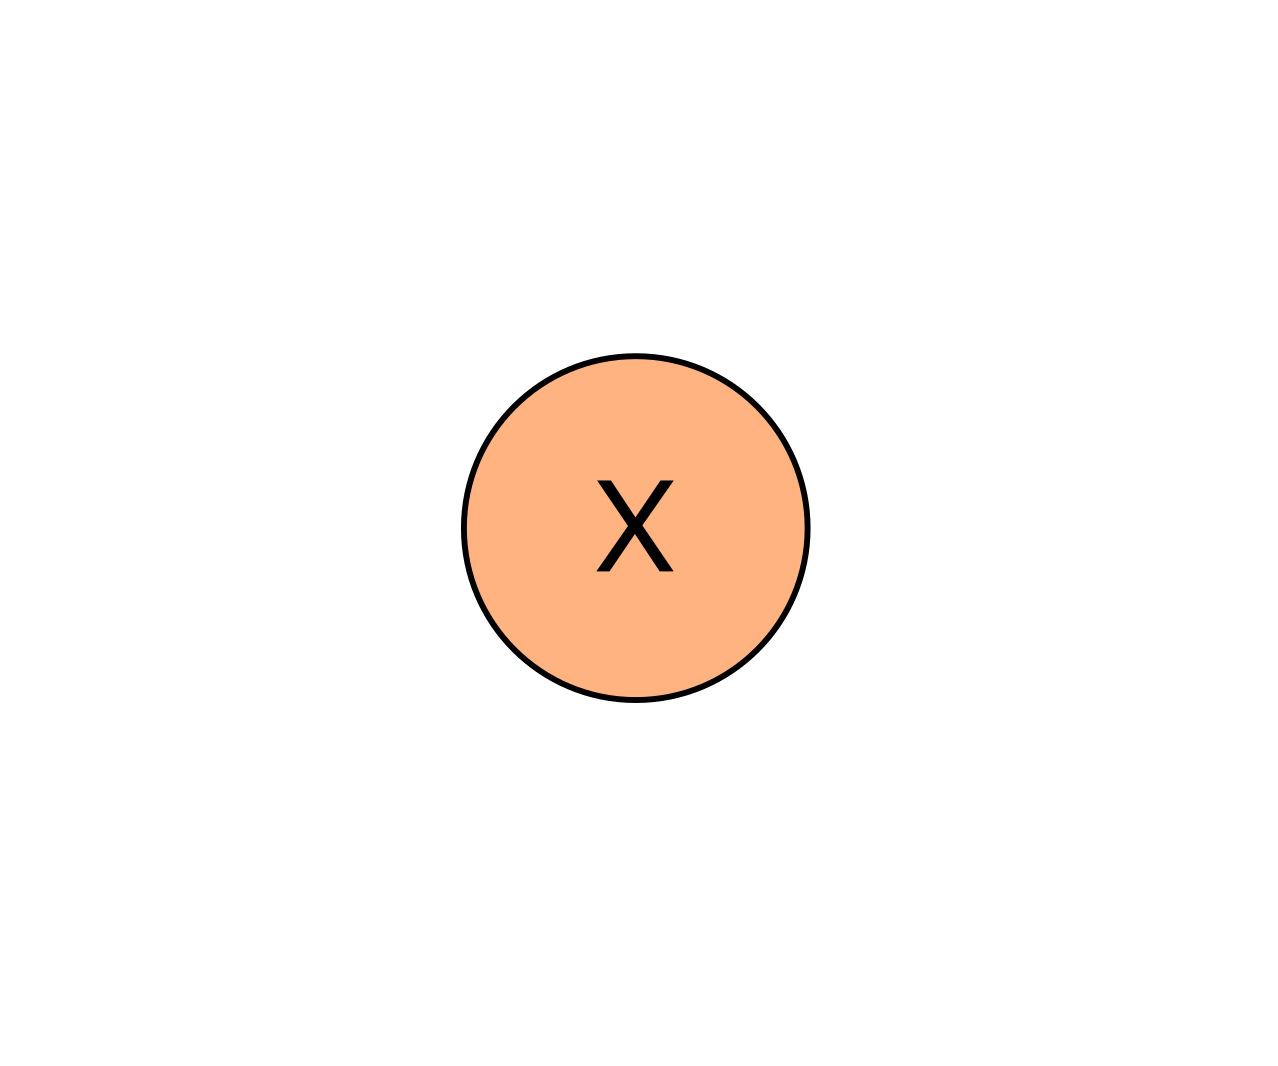
\includegraphics[scale=0.5]{images/neuron.png}
    \caption{Neurônio}
  \end{figure}
  }
  \onslide<2->{%
  Neurônio -- Unidade}
\end{frame}

\begin{frame}{ANN - Unidades e Conexões}%
  \onslide<1->{%
  \begin{figure}[h]{}%
    \label{fig:ann}%
    \centering
    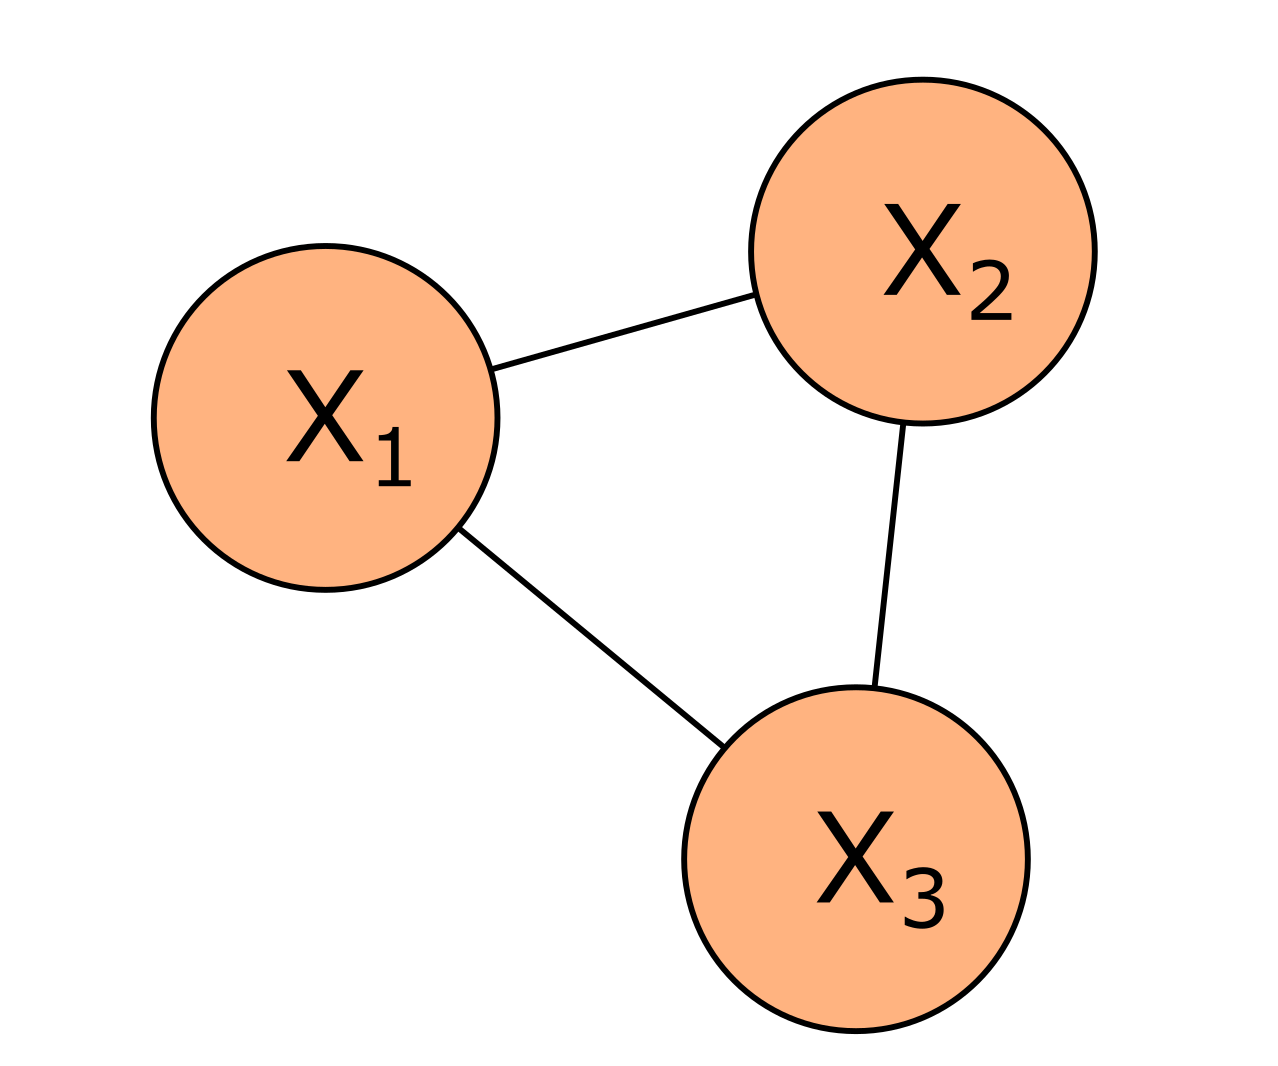
\includegraphics[scale=0.5]{images/ann.png}
    \caption{ANN}
  \end{figure}
  }
  \onslide<2->{%
  Conexões -- Sinápse -- Pesos}
\end{frame}

\subsection{Treinamento e Padrões}%
\begin{frame}{Treinamento e Padrões}%
  \justifying%
  Treinar uma rede neuronal significa determinar o valor das conexões entre as unidades baseado num conjunto de observações que são mostrados para a rede.

  O conjunto de treinamento é composto de padrões, que são estados (configurações) da rede.
\end{frame}
